\section{Specifikationer}
FIR-filteret vælges til at være af type 1, altså er filterordenen $M$ lige og impulsresponsen $h[n]$ er symmetrisk, så $h[n] = h[M - n]$. Filteret har 2 knækfrekvenser $\omega_{c_1}$ og $\omega_{c_2}$ i rad/s, som vælges til at ligge midt imellem henholdsvis $\omega_1$ og $\omega_2$ samt $\omega_2$ og $\omega_3$. Derfor gælder der:
\begin{align*}
\omega_{c_1} &= \omega_1 + \dfrac{\omega_2 - \omega_1}{2} = \frac{\pi}{3} + \dfrac{\pi}{12} = \dfrac{5\pi}{12}, \\
\omega_{c_2} &= \omega_2 + \dfrac{\omega_3 - \omega_2}{2} = \frac{\pi}{2} + \dfrac{\pi}{8} = \dfrac{5\pi}{8}. \\
\end{align*}

\section{Design} \label{ch4_design}
I dette afsnit dokumenteres Python-koden, der anvendes til at filtrere signalet. Først hentes de nødvendige pakker, og herefter defineres henholdsvis filterordenen $M$, længden af filteret $l = M + 1$, en vektor $n$ med $l+1$ heltal mellem 0 og $l$ samt en vektor $x$ med $l+1$ værdier mellem $-\pi$ og $\pi$. Da $\omega_{c_n} = 2\pi f_n$ kan frekvensen $f_n$ i Hz opnås ved relationen $f_n = \frac{\omega_{c_1}}{2\pi}$. Disse definitioner er vist herunder:
\begin{lstlisting}
import numpy as np
import matplotlib.pyplot as plt

M = 200
l = M+1

n = np.linspace(0,l,l+1)
x = np.linspace(-np.pi,np.pi,len(n))

f1 = (5*np.pi/12.) / (2*np.pi)
f2 = (5*np.pi/8.) / (2*np.pi)
\end{lstlisting}

Herefter defineres den ideelle impulsrespons $h_d$ som en funktion, der er 0 mellem $\omega_{c_1}$ og $\omega_{c_2}$ og ellers er 1. Denne udledes i appendix. Denne funktion bruger vektoren $n$, ordenen $M$ samt frekvenserne $f_1$ og $f_2$ i Hz defineret ovenfor. Den ideelle impulsrespons er derfor:
\begin{align*}
h_d[n] = \begin{cases} \dfrac{\sin\left(2 \pi f_1\left(n - \frac{M}{2}\right)\right)}{\pi\left(n - \frac{M}{2}\right)} - \dfrac{\sin\left(2\pi f_1\left(n - \frac{M}{2}\right)\right)}{\pi\left(n - \frac{M}{2}\right)} \quad &\text{for} \quad n \neq \frac{M}{2} \\
1 - 2(f_2 - f_1) \quad &\text{for} \quad n = \frac{M}{2}
\end{cases}
\end{align*}

Dette er implementeret i koden således:
\begin{lstlisting}
def h(n,M,f1,f2):
    hd = np.zeros(len(n))
    for i in range(len(n)):
        if n[i] == M/2:
            hd[i] = 1 - 2*(f2 - f1)
        else:
            hd[i] = (np.sin(2*np.pi*f1*(n[i] - M/2.)) / (np.pi*(n[i] - M/2.))) - (np.sin(2*np.pi*f2*(n[i] - M/2.)) / (np.pi*(n[i] - M/2.)))
    return hd
\end{lstlisting}

Fordi impulsresponsen er endelig skal den ideelle impulsrespons ganges med en vinduesfunktion, der herefter Fourier-transformeres for at opnå en realistisk frekvens- og amplituderespons. Der er forskellige muligheder for denne vinduesfunktion såsom det rektangulære vindue, Hamming-vinduet, Hann-vinduet og Blackman-vinduet. Disse er beskrevet i \cite{side 558-559, DTSP}. Implementeringen af vinduerne i koden er ganske simpel, og som eksempel ses implementeringen af Hann- og Hamming-vinduet herunder:
\begin{lstlisting}
def ha(n,M,a): # Hann-vindue hvis a = 0.5. Hamming-vindue hvis a = 0.54.
    w = np.zeros(len(n))
    for i in range(len(n)):
        if n[i] >= 0 and n[i] <= M:
            w[i] = a - (1 - a)*np.cos((2*np.pi*n[i])/M)
        else:
            w[i] = 0
    return w
\end{lstlisting}

Grafen for Hamming-vinduet er vist på figur \ref{fig:Hamming}.
\begin{figure}[H]
    \centering
    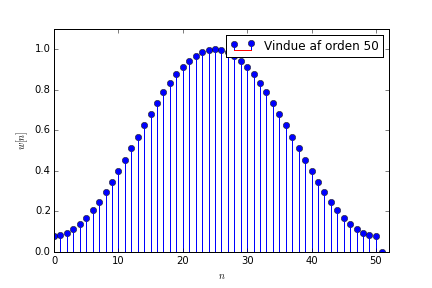
\includegraphics[width = 0.6\textwidth]{figures/Hamming-vindue.PNG}
    \caption{Eksempel på Hamming-vinduet.}
    \label{fig:Hamming}
\end{figure}

Efter implementeringen af vinduerne kaldes funktionerne for den ideelle impulsrespons og det ønskede vindue, som herefter ganges sammen. Dette resultat Fourier-transformeres ved hjælp af den implementerede FFT beskrevet tidligere. Hermed opnås frekvensresponsen $H(e^{j\omega})$, og absolutværdien af dette er amplituderesponsen, som (ideelt set) er 0 mellem $\omega_{c_1}$ og $\omega_{c_2}$ og 1 ellers. Dette afhænger dog især af valget af vinduet og filterordenen $M$. Figur \ref{fig:filter_rekt} viser eksempler på anvendelsen af det rektangulære vindue for $M = 30$ og $M = 100$.

\begin{figure}[H]
\begin{minipage}{0.49\textwidth}
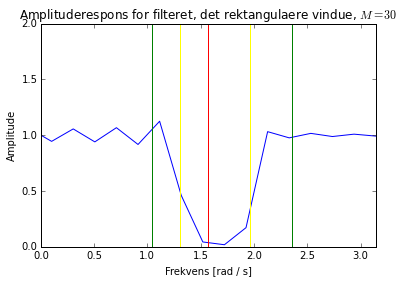
\includegraphics[width=0.9\textwidth]{figures/Filter_rekt_30.PNG}
\end{minipage}
\begin{minipage}{0.49\textwidth}
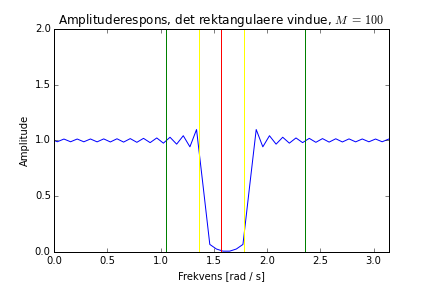
\includegraphics[width=0.9\textwidth]{figures/Filter_rekt_100.PNG}
\end{minipage}
\caption{Eksempler på båndstopfilteret ved hjælp af det rektangulære vindue og med forskellige filterordener $M$. De to grønne streger markerer $\omega_1$ og $\omega_3$, som skal beholdes, og de to gule streger markerer $\omega_{c_1}$ og $\omega_{c_2}$, som ligger symmetrisk omkring den røde streg, der markerer $\omega_2$, som skal elimineres.}
\label{fig:filter_rekt}
\end{figure}

Ud fra figur \ref{fig:filter_rekt} ses det tydeligt, at filteret til en vis grad overholder specifikationerne for begge værdier af $M$, at transitionsbåndet bliver smallere for højere $M$ samt at der er såkaldte ``ripples'' i pasbåndet. Disse ``ripples'' skyldes det rektangulære vindue, der pludselig fra $0$ til $1$ og tilbage igen. For at undgå dette kan man bruge et glattere vindue som for eksempel Hamming-vinduet illustreret på figur \ref{fig:Hamming}.